\documentclass[border=8pt, multi, tikz]{standalone}
%\usepackage{blocks}
\usepackage{import}
\subimport{../../layers/}{init}
\usetikzlibrary{positioning, calc}
\usetikzlibrary{3d} %for including external image 

% \definecolor{KernelColor}{RGB}{0,166,82}
\def\KernelColor{rgb:red,0;green,166;blue,82}
\def\ConvColor{rgb:yellow,5;red,2.5;white,5}
\def\ConvReluColor{rgb:yellow,5;red,5;white,5}
\def\PoolColor{rgb:red,1;black,0.3}
\def\UnpoolColor{rgb:blue,2;green,1;black,0.3}
\def\FcColor{rgb:blue,5;red,2.5;white,5}
\def\FcReluColor{rgb:blue,5;red,5;white,4}
\def\SoftmaxColor{rgb:magenta,5;black,7}


\newcommand{\copymidarrow}{\tikz \draw[-Stealth,line width =0.8mm,draw={rgb:blue,4;red,1;green,1;black,3}] (-0.3,0) -- ++(0.3,0);}

\begin{document}
\begin{tikzpicture}
\tikzstyle{connection}=[ultra thick,every node/.style={sloped,allow upside down},draw=\edgecolor,opacity=0.7]
\tikzstyle{copyconnection}=[ultra thick,every node/.style={sloped,allow upside down},draw={rgb:blue,4;red,1;green,1;black,3},opacity=0.7]

%%%%%%%%%%%%%%%%%%%%%%%%%%%%%%%%%%%%%%%%%%%%%%%%%%%%%%%%%%%%%%%%%%%%%%%%%%%%%%%%%%%%%%%%
%% Draw Encoder
%%%%%%%%%%%%%%%%%%%%%%%%%%%%%%%%%%%%%%%%%%%%%%%%%%%%%%%%%%%%%%%%%%%%%%%%%%%%%%%%%%%%%%%%
\node[canvas is zy plane at x=0] (temp) at (-3,0,0) {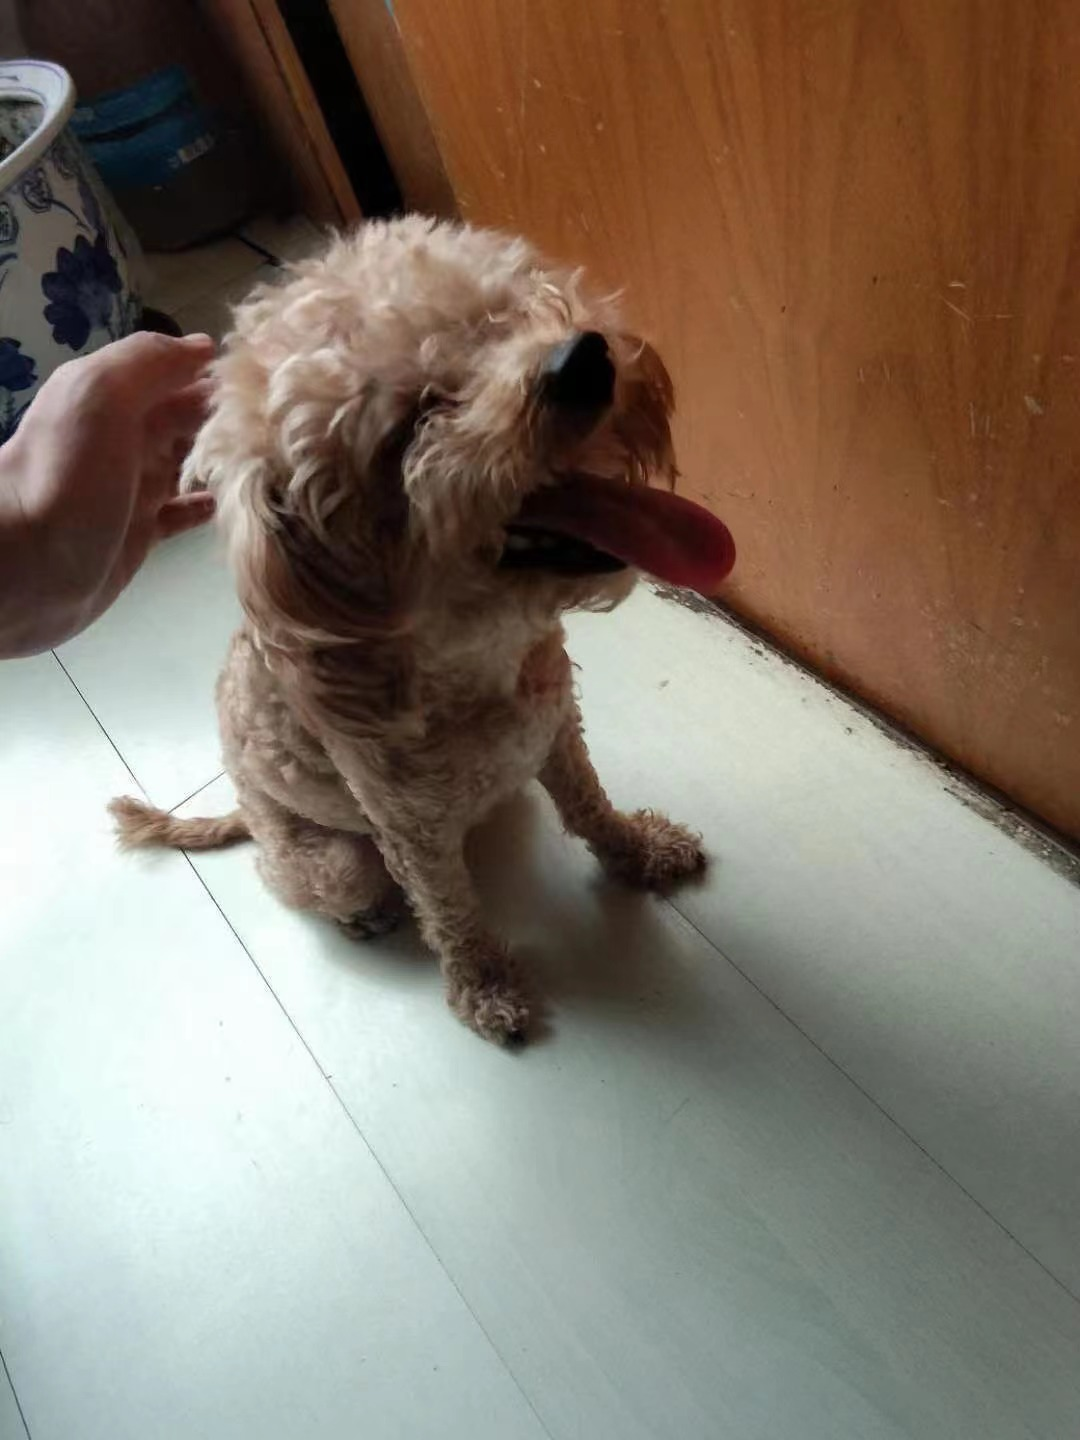
\includegraphics[width=8cm,height=8cm]{Dogs.jpg}};
% conv1 7*7 
\pic[shift={(0,0,0)}] at (0,0,0) 
        {RightBandedBox={
        name=cr1,
        caption=conv1,
        xlabel={{7,}},
        zlabel=7,
        fill=\ConvReluColor,
        height=49,
        width=2,
        depth=49,
        opacity=0.4,
        % % 卷积核参数
        % kernelx=2,
        % kernely=2,
        % kernelz=2,
        % kernelFill=\KernelColor,
        % kernelXLabel={7},   % 设置卷积核的宽度标签
        % kernelYLabel={7},   % 设置卷积核的高度标签
        % % kernelZLabel={112}, % 设置卷积核的深度标签
        % kernelOpacity=0.8,  % 卷积核透明度
        % kernelPos=1         % 卷积核居中
        }
    };   
%%%%%%%%%%
% conv2_x
% maxpool % 3*3 X 2
\pic[shift={(1,0,0)}] at (cr1-east) {
        Box={name=p1,%
        caption=maxpool,
        xlabel={{3,}},
        zlabel=3,
        fill=\PoolColor,
        opacity=0.5,
        height=21,
        width=2,
        depth=21}}; 
\pic[shift={(1,0,0)}] at (p1-east) 
{RightBandedBox={
        name=cr21,
        caption=conv2\_1,
        xlabel={{"3","3"}},
        zlabel=3,
        fill=\ConvColor,
        height=21,
        width={2,2},
        depth=21,
        opacity=0.4,
        }
    };
\pic[shift={(1,0,0)}] at (cr21-east) 
{RightBandedBox={
        name=cr22,
        caption=conv2\_2,
        xlabel={{"3","3"}},
        zlabel=3,
        fill=\ConvColor,
        height=21,
        width={2,2},
        depth=21,
        opacity=0.4,
        }
    };
%%%%%%%%%%
% conv3_x
%  3*3 X 2
\pic[shift={(1,0,0)}] at (cr22-east) 
{RightBandedBox={
        name=cr31,
        caption=conv3\_1,
        xlabel={{"3","3"}},
        zlabel=3,
        fill=\ConvColor,
        height=21,
        width={2,2},
        depth=21,
        opacity=0.4,
        }
    };
\pic[shift={(1,0,0)}] at (cr31-east) 
{RightBandedBox={
        name=cr32,
        caption=conv3\_2,
        xlabel={{"3","3"}},
        zlabel=3,
        fill=\ConvColor,
        height=21,
        width={2,2},
        depth=21,
        opacity=0.4,
        }
    };
% conv4_x
% 3*3 X 2
\pic[shift={(1,0,0)}] at (cr32-east) 
{RightBandedBox={
        name=cr41,
        caption=conv4\_1,
        xlabel={{"3","3"}},
        zlabel=3,
        fill=\ConvColor,
        height=21,
        width={2,2},
        depth=21,
        opacity=0.4,
        }
    };
\pic[shift={(1,0,0)}] at (cr41-east)
{RightBandedBox={
        name=cr42,
        caption=conv4\_2,
        xlabel={{"3","3"}},
        zlabel=3,
        fill=\ConvColor,
        height=21,
        width={2,2},
        depth=21,
        opacity=0.4,
        }
    };
% conv5_x
% 3*3 X 2
\pic[shift={(1,0,0)}] at (cr42-east) 
{RightBandedBox={
        name=cr51,
        caption=conv5\_1,
        xlabel={{"3","3"}},
        zlabel=3,
        fill=\ConvColor,
        height=21,
        width={2,2},
        depth=21,
        opacity=0.4,
        }
    };
\pic[shift={(1,0,0)}] at (cr51-east) {RightBandedBox={
        name=cr52,
        caption=conv5\_2,
        xlabel={{"3","3"}},
        zlabel=3,
        fill=\ConvColor,
        height=21,
        width={2,2},
        depth=21,
        opacity=0.4,
        }
    };


% avgpool
\pic[shift={(1,0,0)}] at (cr52-east) {
        Box={name=p3,
        caption=avgpool,
        fill=\PoolColor,
        opacity=0.5,
        height=7,
        width=1,
        depth=7}};
%%%%%%%%%%%%%%%%%%%%%%%%%%%%%%%%%%%%%%%%%%%%%%%%%%%%%%%%%%%%%%%%%%%%%%%%%%%%%%%%%%%%%%%%
% Draw connections
%%%%%%%%%%%%%%%%%%%%%%%%%%%%%%%%%%%%%%%%%%%%%%%%%%%%%%%%%%%%%%%%%%%%%%%%%%%%%%%%%%%%%%%
\draw [connection]  (cr1-east)    -- node {\midarrow} (p1-west);
\draw [connection]  (p1-east)    -- node {\midarrow} (cr21-west);
\draw [connection]  (cr21-east)    -- node {\midarrow} (cr22-west);
\draw [connection]  (cr22-east)    -- node {\midarrow} (cr31-west);
\draw [connection]  (cr31-east)    -- node {\midarrow} (cr32-west);
\draw [connection]  (cr32-east)    -- node {\midarrow} (cr41-west);
\draw [connection]  (cr41-east)    -- node {\midarrow} (cr42-west);
\draw [connection]  (cr42-east)    -- node {\midarrow} (cr51-west);
\draw [connection]  (cr51-east)    -- node {\midarrow} (cr52-west);
\draw [connection]  (cr52-east)   -- node {\midarrow} (p3-west);

% maxpool中点与conv1中点之间的连接
% 定义两个关键点 betweenpool_2 和 betweencr21_2
\path (p1-east) -- (cr21-west) coordinate[pos=0.75] (betweenpool_2) ;
\path (cr21-east) -- (cr22-west) coordinate[pos=0.25] (betweencr21_2) ;
% 在两个点之间绘制折线连接
% 首先从 betweenpool_2 到 betweencr21_2 添加拐点实现折线效果
% ++(0,-1):然后垂直向下移动 5 个单位,形成第一个 90 度折线。
\draw [connection] (betweenpool_2) -- ++(0,-5) -| (betweenpool_2 -| betweencr21_2) -- node {\midarrow} (betweencr21_2);
% \draw [connection, dashed] (betweenpool_2) -- ++(0,-5) -| (betweenpool_2 -| betweencr21_2) -- node {\midarrow} (betweencr21_2);

% conv2_1与conv2_2中点与 conv2_2与conv3_1中点之间的连接
\path (cr21-east) -- (cr22-west) coordinate[pos=0.75] (betweencr21_22) ;
\path (cr22-east) -- (cr31-west) coordinate[pos=0.25] (betweencr22_31) ;
\draw [connection] (betweencr21_22) -- ++(0,-5) -| (betweencr21_22 -| betweencr22_31) -- node {\midarrow} (betweencr22_31);

%conv2_2与conv3_1中点 与 conv3_1与conv3_2中点之间的连接
\path (cr22-east) -- (cr31-west) coordinate[pos=0.75] (betweencr22_312) ;
\path (cr31-east) -- (cr32-west) coordinate[pos=0.25] (betweencr31_32) ;
\draw [connection, dashed] (betweencr22_312) -- ++(0,-5) -| (betweencr22_312 -| betweencr31_32) -- node {\midarrow} (betweencr31_32);

% conv3_1与conv3_2中点 与 conv3_2与conv4_1中点之间的连接
\path (cr31-east) -- (cr32-west) coordinate[pos=0.75] (betweencr31_322) ;
\path (cr32-east) -- (cr41-west) coordinate[pos=0.25] (betweencr32_41) ;
\draw [connection] (betweencr31_322) -- ++(0,-5) -| (betweencr31_322 -| betweencr32_41) -- node {\midarrow} (betweencr32_41);

% conv3_2与conv4_1中点 与 conv4_1与conv4_2中点之间的连接
\path (cr32-east) -- (cr41-west) coordinate[pos=0.75] (betweencr32_412) ;
\path (cr41-east) -- (cr42-west) coordinate[pos=0.25] (betweencr41_42) ;
\draw [connection, dashed] (betweencr32_412) -- ++(0,-5) -| (betweencr32_412 -| betweencr41_42) -- node {\midarrow} (betweencr41_42);

% conv4_1与conv4_2中点 与 conv4_2与conv5_1中点之间的连接
\path (cr41-east) -- (cr42-west) coordinate[pos=0.75] (betweencr41_422) ;
\path (cr42-east) -- (cr51-west) coordinate[pos=0.25] (betweencr42_51) ;
\draw [connection] (betweencr41_422) -- ++(0,-5) -| (betweencr41_422 -| betweencr42_51) -- node {\midarrow} (betweencr42_51);

% conv4_2与conv5_1中点 与 conv5_1与conv5_2中点之间的连接
\path (cr42-east) -- (cr51-west) coordinate[pos=0.75] (betweencr42_512) ;
\path (cr51-east) -- (cr52-west) coordinate[pos=0.25] (betweencr51_52) ;
\draw [connection, dashed] (betweencr42_512) -- ++(0,-5) -| (betweencr42_512 -| betweencr51_52) -- node {\midarrow} (betweencr51_52);

% conv5_2与avgpool中点 与 avgpool与conv1中点之间的连接
\path (cr51-east) -- (cr52-west) coordinate[pos=0.75] (betweencr51_522) ;
\path (cr52-east) -- (p3-west) coordinate[pos=0.25] (betweencr52_p3) ;
% \path (p3-east) -- (cr1-west) coordinate[pos=0.25] (betweenp3_cr1) ;
\draw [connection] (betweencr51_522) -- ++(0,-5) -| (betweencr51_522 -| betweencr52_p3) -- node {\midarrow} (betweencr52_p3);
%%%%%%%%%%%%%%%%%%%%%%%%%%%%%%%%%%%%%%%%%%%%%%%%%%%%%%%%%%%%%%%%%%%%%%%%%%%%%%%%%%%%%%%
\end{tikzpicture}
\end{document}
